% ==============================================================
\chapter{Introduction}
% ==============================================================

The availability of genome sequences is a key prerequisite for modern 
biological research.
After the discovery of the DNA double helix structure \citep{Watson1953},
genome sequencing techniques have been developed and refined over the decades
\citep{Gilbert1973, Sanger1975}, 
culminating in the publication of the full human genome sequence in 2001 
\citep{Venter2001}.
Aside from the ambiguities introduced by non-coding regions in the genome 
\citep{Gilbert1978} and alternative splicing of genes \citep{Black2003}, 
the genome provides, in theory, all necessary information about which proteins 
can potentially be expressed in a cell.
However, in order to study the dynamic nature of a cell or organism, as for 
example in response to changing environmental conditions, the static information
provided by the genome is not sufficient. 
The transcriptome provides information about gene expression at the RNA level. 
DNA microarray techniques can be employed to screen the regulation of many
genes in parallel on the transcript level \citep{Schena1995}.

Complementing transcriptomics, the field of proteomics deals with the total
set of proteins expressed in a cell, tissue, or organism, at a defined time
point and under certain conditions \citep{Yarmush2002, Yates2009}.
In contrast to transcriptomics, proteomics is situated at the stage of 
translation and protein synthesis, and therefore most accurately reflects the 
phenotype of a cell. 
Mass spectrometry provides an excellent means for proteome analysis
\citep{Aebersold2003}, with speed, accuracy, and sensivity rapidly increasing
within the past two decades.
The major goals of mass spectrometry-based proteomics are protein 
identification and quantitation.
However, since most proteins are too heavy to be measured directly, the
analysis is usually performed on the peptide level, with proteins being digested
prior to the measurement using proteolytic enzymes such as Trypsin, Lys-C, or 
Pepsin. 
The inherent ambiguity introduced by protein isoforms or alternative splicing
poses an additional challenge when peptide identifications are shifted to
the protein level.
In addition to the raw amino acid sequence encoded by a gene, post-translational
modifications play an important role in defining the actual function of a
protein.
Post-translational modifications may modify a protein by adding an enzyme or by
chemically modifying certain residues.
Furthermore, structural adjustments such as the formation of disulfide 
bonds between Cysteine residues may be required for the protein to become 
functional.
Employing mass spectrometry, it is possible not only to identify peptides and
proteins, but also to study their various modifications.
Another application of mass spectrometry-based analysis is the localization of
proteins to certain compartments of a cell, for example by semi-quantitative
analysis.

Although modern mass spectrometers are very sensitive, a couple of sample 
preparation steps must be carried out in order to achieve comprehensive 
proteome coverage. 
An example of a mass spectrometry-based proteomics workflow for peptide 
and protein identification is depicted in Fig.~\ref{fig:proteomics-overview}.

\begin{figure}
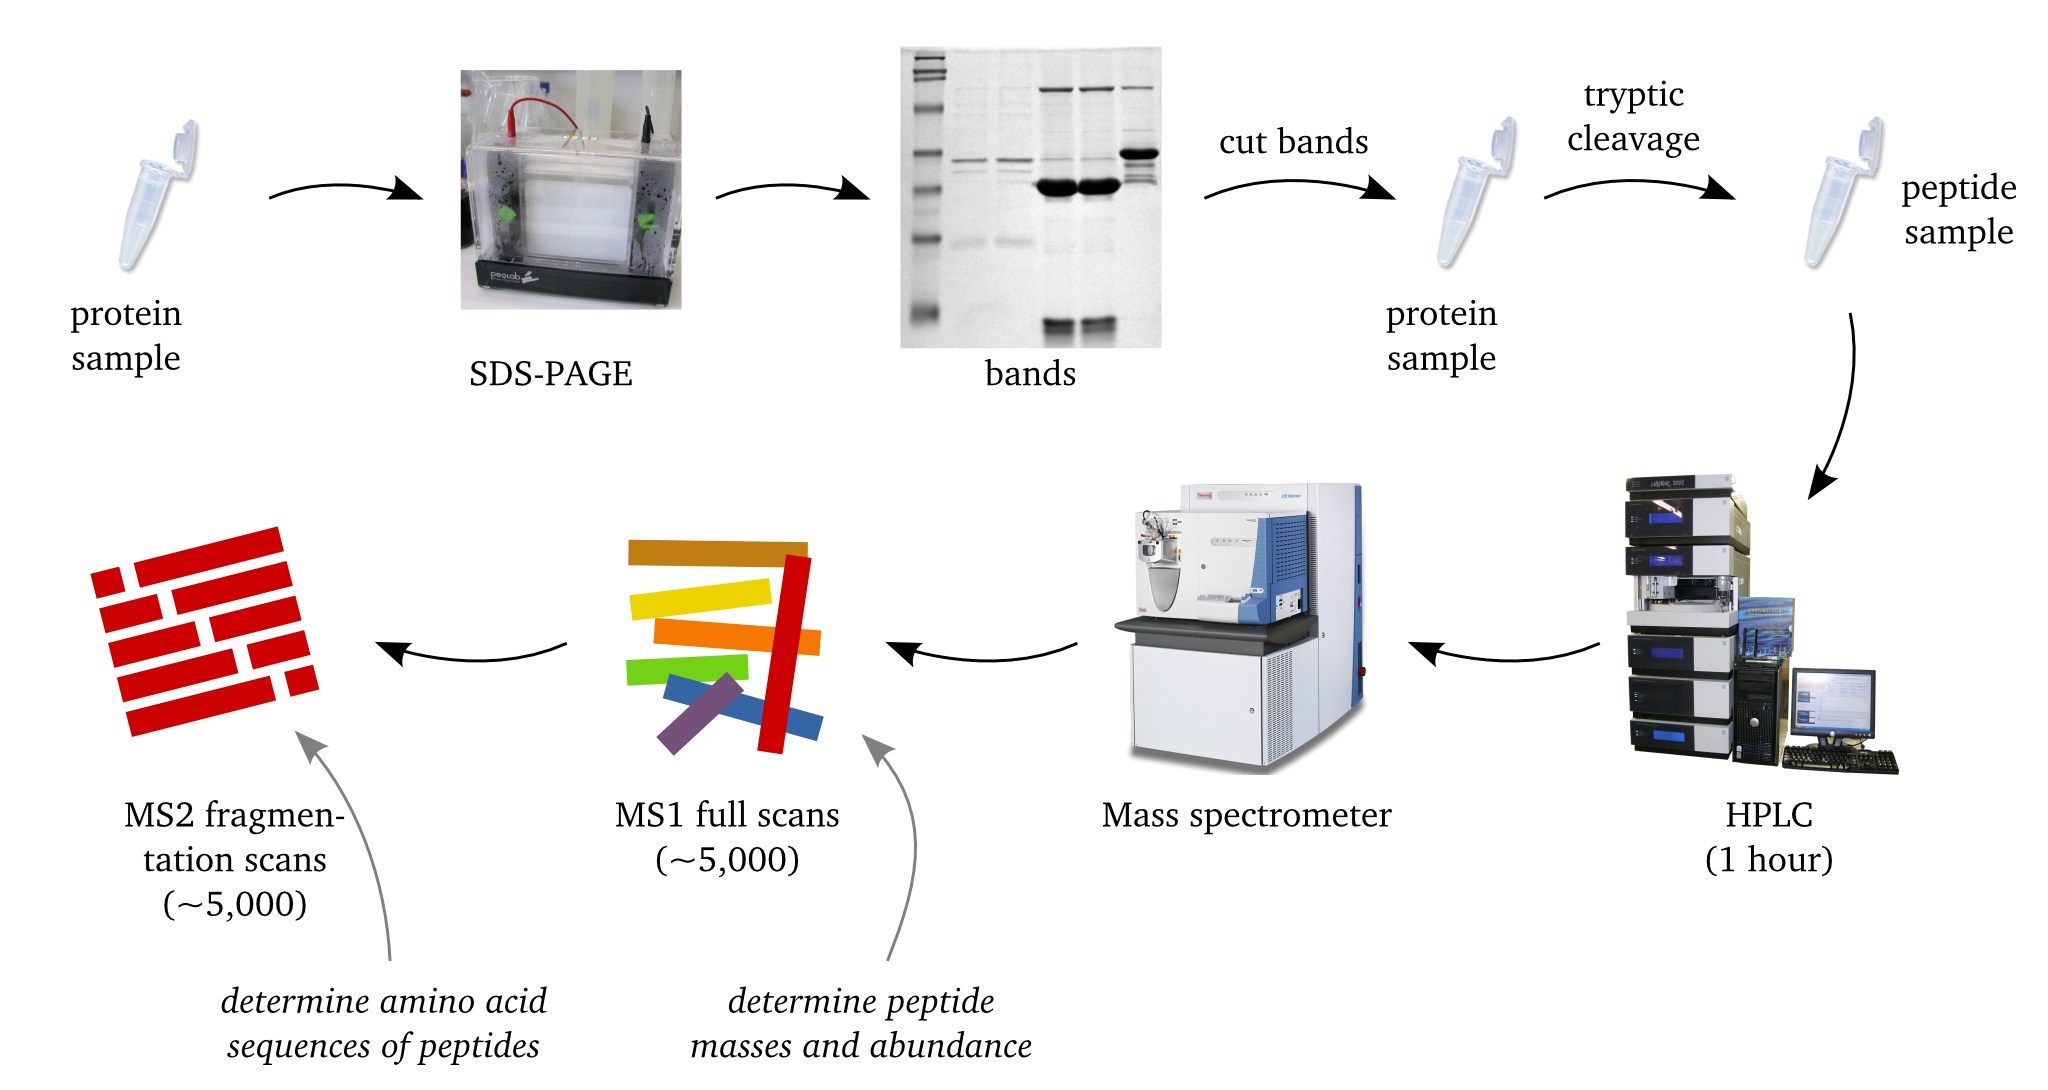
\includegraphics[width=\textwidth]{figures/Proteomics.jpg}
\caption{
{\bf Example of a mass spectrometry-based proteomics experiment workflow.} 
Protein samples are fractionated via SDS-PAGE and resulting bands are excised and
digested proteolytically. In order to further separate the complex mixture, 
the resulting peptides are loaded onto a HPLC column and subsequently eluted 
and injected into the mass spectrometer. Full scans and fragmentation scans
are recorded as peptide elution is in progress for a pre-defined amount of time.
}
\label{fig:proteomics-overview}
\end{figure}

% --------------------------------------------------------------
\section{Acquisition of mass spectrometric data}
% --------------------------------------------------------------

In the following, the steps involved in the acquisition of mass spectrometric
data are described.

\subsection{Preprocessing of biological samples}

Although mass spectrometric analysis of intact proteins has been successfully
reported \citep{Lee2002, Taylor2003}, such an approach is not feasible in 
general because the high mass of proteins cannot be accounted for with most
types of mass spectrometers.
In addition, low abundant proteins may be missed in complex samples due to
the fact that there are many more highly abundant proteins present.
To overcome these obstacles, a couple of sample preprocessing steps are usually
undertaken, with possible variations depending on the experimental context.

\subsubsection{Gel electrophoresis}

Due to the high dynamic range of protein expression levels, complex protein 
mixtures tend to produce less comprehensive results because low abundant 
proteins are `shadowed' by highly abundant proteins. 
Gel electrophoresis may be used as a first sample separation step in which
proteins are ordered by size, resulting in a number of fractions which can
be analyzed individually.
For SDS-PAGE, a sodium dodecyl sulfate polyacrylamide gel is prepared and
proteins are loaded into wells in the gel.
An electric field is applied to the gel, thus inducing an electromotive force 
on the proteins which move through the gel at a speed which depends on their
size and charge.
However, SDS leads to denaturation of proteins and results in an overall
negative charge for all proteins. 
Thus, the migration speed of the proteins is only dependent on their size. 
Individual spots of equally-sized proteins may be visualized using Coomassie 
dye and subsequently excised.

In order to achieve even higher sample separation, two-dimensional gel 
electrophoresis may be used \citep{Klose1975, O'Farrell1975}.
Here, proteins are additionally separated by a second physicochemical property
such as their isoelectric point.
As in the SDS-PAGE approach, resulting spots may be excised and subjected 
to mass spectrometric analysis.

\subsubsection{Proteolysis}

In order to break proteins up into small, mass spectrometry-compatible peptides, 
proteolytic enzymes are used.
Among the various choices of possible enzymes, Trypsin has become very popular
because it results in short peptides with a basic residue at the C-terminus
\citep{Olsen2004}.
Trypsin cleaves specifically at the C-terminal side of Lysine and Arginine 
residues, given that no Proline residue is located at the other side of the 
cleavage site.
Alternative enzymes such as Asp-N and Glu-C are sometimes used to generate
complementing peptides which overlap with the tryptic peptides in order to 
increase sequence coverage of peptide identifications \citep{Steen2004}.
Although Trypsin, Asp-N and Glu-C are very sequence-specific, the possibility 
of missed cleavage sites must be taken into account during data analysis.

\subsubsection{Liquid chromatography}

In addition to fractionation via SDS-PAGE, liquid chromatography (LC) provides 
a second dimension of separation, usually at the peptide level.
For the experiments covered in this thesis, a reverse phase liquid 
chromatography (RPLC) system has been employed.
In this setup, peptides elute according to their hydrophobicity.

\subsection{Ionization of molecules}

In order to make molecules suitable for mass spectrometric analysis, 
the analyte must be ionized and transferred to the gaseous phase.
Among many available options, the two most widely used methods for this 
task are (1) matrix-assisted laser desorption/ionization (MALDI) for solid 
analytes, and (2) electrospray ionization (ESI) for liquid samples.
% MALDI
In the MALDI approach \citep{Karas1988}, the analyte is mixed with a 
matrix material and co-cristallized on a metal plate. 
A pulsing laser beam is used to excite the matrix and sublime several 
contained analyte molecules. 
Although initially, mostly matrix molecules get ionized by the laser
beam, charges are transferred to the analyte molecules while the
matrix/analyte cloud is moved towards the mass analyzer by an
electric field.
% ESI
ESI provides the advantage that it can be directly coupled to an
upstream LC system because it works with fluid samples \citep{Fenn1989}.
Here, the sample is pumped into a spray needle, either from the LC or via
direct injection. 
A high potential is applied between the entrance of the mass spectrometer and
the tip of the spray needle, resulting in electrostatic dispersion of the
effluent as it exits the needle tip.
The resulting charged droplet evaporates into smaller droplets until finally,
in the best case, only one analyte ion is contained in a single droplet.

\subsection{Mass analysis and ion detection}

Regardless of the ionization process, several options are available for
the most prominent part of a mass spectrometer, the mass analyzer.
% TOF
In the time-of-flight (TOF) mass analyzer \citep{Wolff1953}, equally charged 
ions are accelerated to the same kinetic energy, resulting in a velocity 
which is dependent on the {\em m/z} value of an ion, with lighter ions
moving faster than heavier ions.
The time required for the ion to hit the ion detector is measured and
then converted to the corresponding {\em m/z} value.
% Quadrupole
In the quadrupole mass analyzer \citep{Paul1956}, four parallel rods are 
used to create a radio frequency quadrupole field which can be controlled
in such a way that only ions of a specified mass-to-charge ratio can pass.
For the creation of a mass spectrum, the {\em m/z} range is traversed from
minimum to maximum and the passing ions are recorded.

% Ion traps

The third type of mass analyzer discussed in this thesis is the ion trap,
which is available in a couple of variants.
Common to all ion traps is that lower analyte amounts are required as
compared to quadrupole mass analyzers, because instead of scanning
the entire {\em m/z} range as the sample passes through the mass spectrometer 
and discarding all ions which do not match the current {\em m/z} value, 
ions are first trapped and collected in the ion trap and then ejected 
sequentially, traversing the entire {\em m/z} range.
In the three-dimensional quadrupole ion trap, ions are trapped in a space
confined by a ring electrode and two endcap electrodes.
The linear ion trap uses a two-dimensional field and provides for higher ion
storage capacity, resulting in an increased detection sensitivity.
The Fourier transform ion cyclotron resonance (FT-ICR) mass analyzer provides
for extremely high mass resolution which.
However, a strong magnetic field must be created and sustained, resulting
in high maintenance as the system needs to be constantly cooled with helium. 
The most recent development in this area, the Orbitrap, combines high mass 
accuracy with low maintenance requirements \citep{Hu2005}. 
A Thermo Scientific LTQ Orbitrap XL mass spectrometer has been used for the
acquisition of all mass spectrometric data used in this thesis.

Another aspect of ion traps is that fragmentation of previously selected,
specific precursor ions becomes possible.
This is a prerequisite for tandem mass spectrometry (MS/MS), or data dependent
acquisition.
Here, a pre-defined, fixed number of highly abundant precursor ions is selected
from every full scan, and subsequently subjected to fragmentation
in a process called {\em collision induced dissociation} (CID).
Here, peptides collide with an inert gas and subsequently break apart into 
N- and C-terminal fragments, thereby producing {\em b} ions and {\em y} ions, 
respectively. 
Depending on the actual fragmentation site within the peptide bond,
alternative fragment ions may result: {\em a} and {\em c} ions for N-terminal
fragments, {\em x} and {\em z} ions for C-terminal fragments.

\subsection{Mass spectra}

Recorded mass spectra are stored as vendor-specific files which contain meta 
information which describes the acquired data as well as the raw peak data.
In order to unify the exchange of mass spectrometers raw data, the mzML file 
format has been devised by the HUPO Proteomics Standards Initiative
\citep{Deutsch2008}.
Apart from the file format details, several different scan types can be
acquired, each of which contains different information.

\subsubsection{Full scans (MS)}

Full scans provide an overview over the peptides which are present in the
mass spectrometer at a given time (see Fig.~\ref{fig:full-scan}).
The \mz~values of all intact peptides are reported.
However, the absence of a precursor peak does not necessarily indicate the
absence of the corresponding peptide in the sample, because detection of
an ion may fail for various reasons.
Following a full scan, one or more highly abundant precursors are usually
selected for further analysis.

\begin{figure}[h]
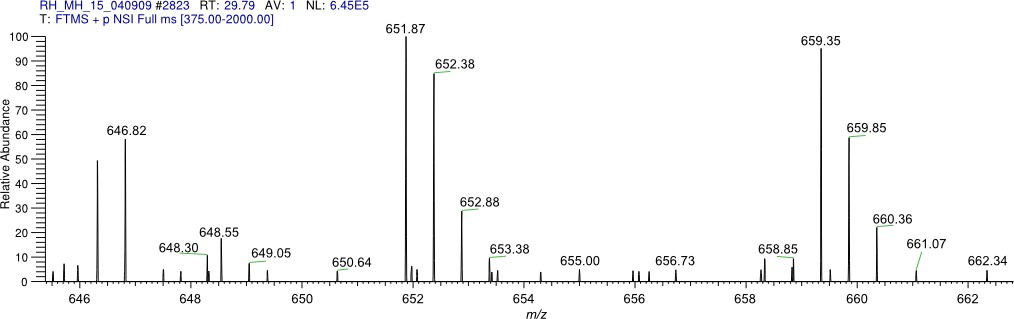
\includegraphics[width=\textwidth]{figures/ms1-scan.jpg}
\caption{
{\bf Zoomed view of a full scan.}
Isotope envelopes of doubly charged peptides, consisting of precursor
peaks with a \mz~difference of $\sim0.5$ are visible,
}
\label{fig:full-scan}
\end{figure}

\subsubsection{Fragmentation scans (MS/MS)}

The scans resulting from collision-induced dissociation are called 
fragmentation scans, or tandem MS (MS/MS) scans.
From the observed fragment ions, {\em mass ladders} can be constructed which
represent the amino acid sequence of the selected peptide (see Fig~\ref{fig:fragmentation-scan-b-y}). 
When fragmentation peaks are missing, the exact sequence of the peptide may not
become clear from a single mass ladder.
However, a combination of multiple mass ladders can resolve such ambiguities.

\begin{figure}[h]
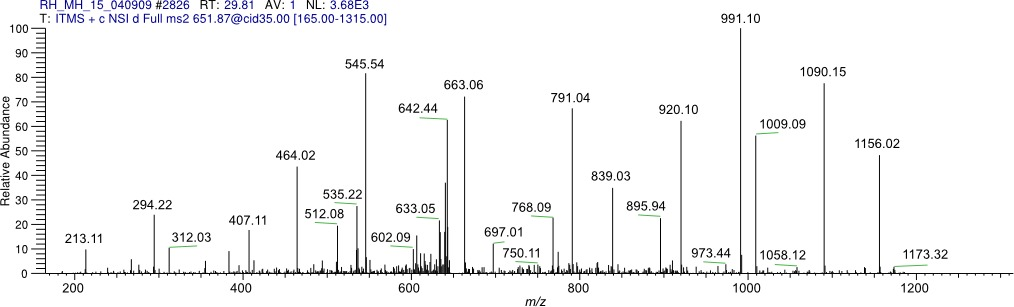
\includegraphics[width=\textwidth]{figures/ms2-scan.jpg}
\caption{
{\bf Example of a fragmentation scan.} 
The 651.87 \mz~precursor peak shown in Fig.~\ref{fig:full-scan} has been
subjected to collision-induced dissociation.
Resulting fragment ions are recorded in the fragmentation scan.
}
\label{fig:fragmentation-scan}
\end{figure}

\begin{figure}[h]
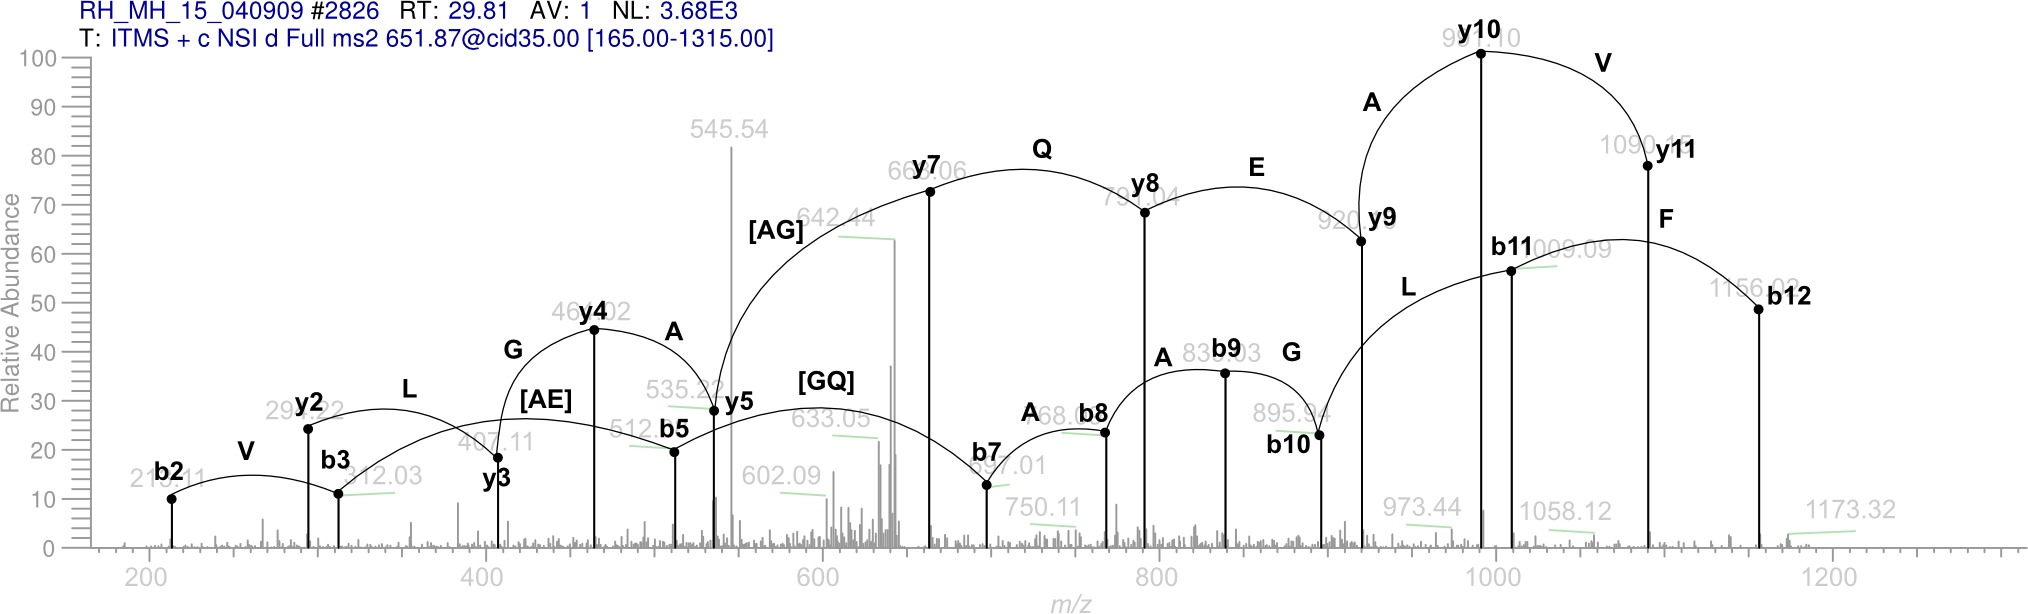
\includegraphics[width=\textwidth]{figures/ms2-scan-b-y-1.jpg}
\caption{
{\bf The MS/MS scan depicted in Fig.~\ref{fig:fragmentation-scan} with {\em b} and 
{\em y} ion series mass ladders superimposed.} 
The \mz~differences of fragmentation peaks reflect the masses of individual amino
acids or short amino acid oligomers.
}
\label{fig:fragmentation-scan-b-y}
\end{figure}


% --------------------------------------------------------------
\section{Mass spectrometric data evaluation}
% --------------------------------------------------------------

Evaluation of the acquired mass spectrometric data is a process with a multitude
of possible options.
Usually, the decisions made during sample preparation and data acquisition are
reflected in the data analysis: If proteins were separated via SDS-PAGE, the
resulting order of proteins via their mass can be used to verify or falsify 
identifications.
Likewise, if liquid chromatography is employed, the retention time at which
peptides have been identified can be used for plausibility checks.

Sequence databases, including genome and protein sequences, play an important
role in MS/MS data evaluation because they greatly confine the search space
for peptide identification from MS/MS spectra.
However, care must be taken if these databases are not comprehensive, because
the search space defined by incomplete sequence databases might be too small
to provide for proper identification.


\subsection{Identification}

Several possibilities have been established to identify peptides present
in the sample. 
Usually, only a fraction of all peptides present in a sample can be 
identified for various reasons.
Firstly, peptides stemming from low abundant protein may be missed because 
they result in low precursor peaks which are generally less favored, and
therefore harded to detect, when compared to high peaks that can be clearly
distinguished from noise peaks.
Another problem arises when highly complex samples are used and the
high number of peptides outnumbers the number of scan events in the
mass spectrometric run.
Also, highly abundant peptides are prone to be identified repeatedly,
thus decreasing the identification chances of low abundant peptides.
Finally, the differing physicochemical properties of all peptides
lead to the effect that only a subset of the sample can be ionized and
fragmented in such a way that identification is possible.

\subsubsection{Peptide mass fingerprinting}

Peptide mass fingerprinting is a protein identification method which was
simultaneously developed by several groups in 2003 
\citep{Henzel1993,James1993,Mann1993,Pappin1993a,Yates1993}.
In this method, the observation of several intact peptide precursor masses
(the peptide mass fingerprint) is used to identify the protein which was 
present in the sample.
Peptides are determined {\em in silico} prior to the search from a protein
database and their masses are subsequently matched to the observed precursor
peaks.
Accoring to \citet{Mann1993}, four to six proteolytic peptides measured
at a mass accuracy between 100 and 1,000 ppm are usually sufficient to
characterize a protein.
The acquisition and interpretation of fragmentation is scans is not required, 
however the method has the disadvantage that only samples containing a single 
protein can be analyzed and complex protein mixtures cannot be used.

\subsubsection{Database search}

One year after the advent of the peptide mass fingerprint approach, a novel
method for the identification of peptides was developed by \citet{Eng1994}.
In their study, \citeauthor{Eng1994} introduced SEQUEST, an algorithm which
takes fragmentation scans and a protein sequence database as input files.
From the protein sequences, {\em in silico} digested peptides are determined
and their theoretical fragmentation scans predicted.
Finally, using the precursor mass as a first filtering criterion, all
theoretical and measured fragmentation scans are compared via cross-correlation
and the resulting matches are scored and ranked.
Subsequently, the best matching peptide is regarded as the correct 
identification of the corresponding fragmentation scan, given that there is
no different, competing identification with a similarly good score.
This prerequisite for the correctness of peptide identifications highlights
a drawback of the method: as for peptide mass fingerprinting, the peptide
identification completely depends on the protein sequence database used.
Sequences which are not covered by the database are not tested and therefore
cannot weaken the identification distinctness of a particular peptide/spectral 
match (PSM).
In the recent years, several new database search programs have become 
available, including MASCOT \citep{Perkins1999}, X! Tandem \citep{Craig2004},
OMSSA \citep{Geer2004}, and MyriMatch \citep{Tabb2007}.

Initially, individual peptide/spectral matches had to be validated manually,
and consensus score thresholds could be used as a rough estimate to distinguish
incorrect from correct peptide identifications.
With the advances in mass spectrometry leading towards high-throughput analyses,
such an approach was no more feasible and a method for the assessment of
the statistical significance of peptide/spectral matches was required.
Two methods were developed for this purpose: 
In \citeyear{Keller2002}, \citeauthor{Keller2002}~proposed an algorithm which
assumes the score distribution from a set of 
peptide/spectral matches to be composed of two distinct distributions,
one for incorrect, and one for correct assignments. 
The algorithm presented in their study \citep{Keller2002}, PeptideProphet,
attempts to disentangle these distributions and separate false from correct
identifications.
An alternative approach which is very flexible and easy to implement was
proposed five years later by \citeauthor{Elias2007}.
In their paper, the authors proposed a target/decoy search strategy to 
facilitate posterior probability estimation of the complete list of
peptide/spectral matches resulting from a database search \citep{Elias2007}.
To achieve this, the input protein database is complemented with an equally 
sized {\em decoy database} which contains sequences derived from the original
database entries by reversing or shuffling the amino acid sequence.
To the database search program, peptides from both target and decoy sequences 
appear as equal candidates to explain fragmentation scans.
From the resulting of list of assignments, a score threshold can be determined
in such a way that a user-defined estimated false discovery rate (FDR) is
achieved in regard to the complete set of identifications.
In practice, the score threshold is determined by traversing the entire PSM 
list, starting from the best-scoring assignment and counting the number
of true (target) and false positive (decoy) hits.
Based on these numbers, \citeauthor{Elias2007} estimate the FDR as

\begin{equation}
\text{FDR} = \frac{2 \cdot n_{\text{decoys}}}{n_{\text{targets}} + n_{\text{decoys}}}.
\end{equation}

\citeauthor{Kall2008a} propose an alternative FDR estimation 
\citep{Kall2008a}:

\begin{equation}
\text{FDR} = \frac{n_{\text{decoys}}}{n_{\text{targets}}}.
\end{equation}

Regardless of the actual estimation, the target/decoy approach is based on 
the following assumptions \citep{Elias2007}: (1) proteolytic peptides inferred 
from the target and decoy databases do not overlap, and (2) false positive 
identifications from both databases are equally likely.
These requirements have implications for the creation of the decoy sequences
and as a consequence, there is an upper database size limit for which the 
target/decoy approach is feasible.

\subsubsection{{\em De novo} sequencing}

For the interpretation of fragmentation scans, {\em de novo} sequencing is
a highly unbiased method.
Here, the mass ladders recorded in a fragmentation scan are reconstructed
and a list of full peptide sequence candidates is returned as a result.
Because the assignment of peptides to fragmentation spectra does not rely
on a sequence database, the identifications are unbiased and especially
useful for organisms with unsequenced genomes or incomplete genome sequences.
Due to the inherent ambiguities regarding the interpretation of fragmentation
peaks and their assignment to {\em b} or {\em y} ion mass ladders, and the 
problem of interfering noise peaks, interpretation is difficult and 
high-resolution spectra are usually required to achieve correct results.
In addition, the speed of such algorithms is generally very low because the
search space is only confined by the proteolytic enzyme which was used
for protein digestion and apart from that, all possible amino acid sequences
must be taken into account.
Available {\em de novo} sequencing programs include Lutefisk 
\citep{Johnson2002}, PEAKS \citep{Ma2003} and PepNovo \citep{Frank2005}.

A common problem with {\em de novo} sequencing is that the resulting peptides
are generally not completely correct across the entire amino acid sequence, 
and an automated method to validate peptides and use the resulting validated 
peptides in a downstream analysis is not readily available. 
Therefore, {\em de novo} sequencing is often used as a complementing method 
which is used in special cases and requires manual verification.
A hybrid approach combining {\em de novo} sequencing and database search
is implemented by sequence tag search algorithms such as InsPecT 
\citep{Tanner2005} or ByOnic \citep{Bern2007}.
Here, short sequence tags, consisting of a short amino acid sequence and the
masses of the N- and C-terminal fragments are extracted from the fragmentation 
spectrum.
The subsequent database search is restricted to the peptides which match
the extracted sequence tag, thereby increasing search speed.

\subsubsection{Genomic Peptide Finder}

The Genomic Peptide Finder (GPF), originally devised by \citeauthor{Allmer2004} 
in \citeyear{Allmer2004}, follows a different strategy for the use of 
{\em de novo} predicted amino acid sequences \citep{Allmer2004}.
Instead of matching short sequence tags to gene model proteins, GPF uses the
six frame translation of a genomic DNA sequence as a matching target.
From a given {\em de novo} sequenced peptide, all sequence tags of a 
user-defined size are extracted and each of the sequence tags is located
within the six frame translation.
From the resulting locations, the deduction of candidate peptides is attempted,
each of which could be a possible explanation of the fragmention scan the
{\em de novo} sequenced peptide originated from.
All deduced candidate peptides fulfill the following criteria:

\begin{itemize}
\item a short sequence tag (typically three to five amino acids) has been 
correctly predicted via {\em de novo} sequencing 
\item the position of the sequence tag within the peptide, as defined by
either the N- or C-terminal fragment mass, is correct within the limits 
defined by the fragment scan mass accuracy (typically 700 ppm for an ion trap)
\item the total mass of the peptide matches the observed precursor mass
within the range defined by the full scan mass accuracy (typically 5 ppm for 
the Orbitrap)
\end{itemize}

In addition to unspliced candidate peptides, the deduction of spliced candidate
peptides is attempted by considering a user-defined maximum intron length.
The resulting peptides may then be used to verify or falsify existing gene 
models, as shown in a subsequent publication where GPF was used to confirm 
2174 gene model peptides and further identify 448 novel peptides, including 98 
spliced peptides \citep{Allmer2006}.
The manual inspection of the identified peptides lead to the identification
of novel gene models, the improvement of existing gene models as well as 
hints for alternative splicing.

In 2007, GPF was redesigned and implemented from scratch in the scope of this
thesis to add a variety of features \citep{Specht2011_GPF}:

\begin{itemize}
\item intron splits may occur within a single coding nucleotide triplet
\item splice donor/acceptor site consensus sequences may be specified to
reduce the number of spurious spliced peptide alignments
\item increased search speed by employing an indexing strategy while locating
the occurences of sequence tags in the genomic DNA sequence
\end{itemize}

In addition, a method for the automated validation of GPF candidate peptides,
employing standard database search programs such as OMSSA was established.
This allows for statistically robust identification of GPF-deduced peptides
alongside gene model peptides.
Furthermore, an annotation pipeline was established in which resulting GPF
peptides are passed to AUGUSTUS, which performs an {\em ab initio} gene 
model prediction supplemented by various extrinsic hint sources including
GPF peptides.
It is therefore a major contribution of this thesis that an automated
proteogenomic annotation of the \cre~genome in which MS/MS data generated
for various unrelated purposes can be re-used for the generation of
extrinsic AUGUSTUS hints has become possible.

\subsection{Quantitation}

In addition to determining which peptides, and therefore proteins, are 
contained in a sample, it is often of interest to determine the abundance
of proteins in samples from different conditions \citep{Schulze2010}.
Using this information, the effect of various influences, such as environmental 
stress or periodic environmental changes such as the light-dark cycle,
can be elucidated.
Generally, two samples are compared in one experiment and in most approaches, 
quantitation results are relative, indicating up-regulation, down-regulation 
or unchanged abundances for various proteins.
If a standard of known amount is spiked into the sample and quantified alongside
the proteins of interest, these relative results can typically be promoted to 
absolute quantitation results.

\subsubsection{Chemical labeling}

Chemical labeling methods introduce a label into the peptides from one of the 
samples via a chemical reaction. 
The {\em isotope-coded affinity tag} method (ICAT) 
uses two affinity tags {\em d0} and {\em d8} which bind to cysteine residues
and introduce a mass shift of 0 and 8 Da, respectively \citep{Gygi1999}.
The mass shift of 8 Da can be observed in the full scans and the area under
the respective precursor ion isotope envelopes can be used to estimate
the ratio of peptide abundance in both samples.
However, because the method is restricted to mass spectrometry-compatible 
peptides which contain a cysteine residue, ICAT yields comparably low proteome
coverage.

The {\em isobaric tag for relative and absolute quantitation} method (iTRAQ)
follows a similar approach by introducing isobaric tags into the peptides in
different samples \citep{Ross2004} at the stage of enzymatic digestion.
However, the N-terminus of peptides is labeled, resulting in increased proteome
coverage.
Each iTRAQ tag consists of a reporter group and a balance group, which together 
result in a mass shift of 145 Da. 
However, several distinct tags are available and possible reporter group masses 
include 114 Da, 115 Da, 116 Da, and 117 Da, thus enabling the simultaneous 
analysis of more than two samples (an iTRAQ variant with 8 different tags is also
available).
The isobaric tags result in the effect that equal peptides from different 
samples appear at the same {\em m/z} value in the full scan.
During fragmentation, the reporter groups get separated from the peptide, 
resulting in distinct reporter peaks in the fragmentation scan, allowing
for subsequent quantitation of peptides identified via tandem mass spectrometry.
In comparison to the ICAT method, peptide quantitation is only performed in 
fragmentation scans and therefore the amount of sampled quantitation ratios 
per peptide is usually low.

\subsubsection{Metabolic labeling}

As an alternative to chemical labeling, metabolic labeling can be used for
peptide and protein quantitation in organisms which can be forced to incorporate
an isotopically labeled amino acid or a stable isotope of a certain chemical 
element.
In this approach, the label is introduced via the metabolism of an organism.
In the {\em stable isotope labeling with amino acids in cell culture} method
(SILAC), strains are required which are not able to synthesize certain amino
acids such as Arginine or Lysine \citep{Ong2002}.
For \cre, the Arginine-auxotrophic strain CC424 is available which
must be supplied with Arginine to survive.
The fact that $^{13}$C-labeled Arginine exposes the same physicochemical 
properties as the natural $^{12}$C Arginine and thus the organism is 
oblivious to the isotopically labeled variant can be used to create 
unlabeled and labeled samples which can later be mixed and measured in a 
single MS/MS experiment.
Using tryptic peptides and a $^{13}$C-Arg label, a mass shift of 6 Da is 
typically introduced for each peptide because one Arginine amino acid 
contains six carbon atoms.
Due to the physicochemical equality of sister peptides in the mixed sample,
equal peptides from both conditions can be expected to co-elute and therefore
appear next to each other in several full scans. 
From peptide identifcations in nearby fragmentation scans, the identity of
sister peptide precursor peaks can be assumed and subsequently, the peptide
can be quantified.
In the case of $^{13}$C-Arg labeling, only 50\% of all tryptic peptides can
be expected to be suitable for quantitation, because trypsin cleaves C-terminal
of Arginine and Lysine residues, resulting in roughly half of all tryptic 
peptides containing no Arginine at all.
However, different variations are possible, for example, $^{13}$C-Arg/Lys 
labeling can be used, although this requires a strain which is both Arginine
and Lysine-auxotrophic.

\subsubsection{Label-free quantitation}

In the recent years, label-free quantitation methods have been developed and
constantly refined.
In these approaches, no labels are required and measurements of two or 
more samples are cross-correlated to determine relative peptide and protein
amounts in the respective conditions.
Spectral counting is a coarse and simple way of assessing protein ratios by
comparing the number of scans a peptide, and therefore protein, was identified
in across the various samples \citep{Old2005}.
Given that a minimum number of peptide/spectrum matches could be obtained from
each sample, a rough estimation of the protein ratio can be carried out.
However, it must be taken into account that the number of triggered and
subsequently identified scans depends on many factors.
In addition, if a dynamic exclusion filter is employed during the measurement 
to disable re-triggering of the same highly abundant precursor {\em m/z} value 
for a certain time (typically 90 seconds), this effect must be taken into 
account when peptide abundance is inferred from the number of scans the peptide
has been identified in.

\begin{todo}
across several runs
\end{todo}

\section{Proteogenomics}
\label{proteogenomics}

Genome sequence databases are a prerequisite for the prediction of protein 
databases, and full genome sequences for more than 180 species are available
\citep{Yates2009}.
The annotation of genomic sequences remains a challenge, especially in
eukaryotic genomes, where protein coding sequences are interrupted by
introns.
% EST support
Various strategies have been proposed to identify protein coding genes in
genomic sequences using expressed sequence tags (EST) libraries, 
including the UCSC KG II \citep{Karolchik2003}, ENSEMBL \citep{Hubbard2005} 
and NCBI Gnomon annotation pipelines \citep{Maglott2005}.
In this method, genes are identified by mapping known cDNA tags to the
genomic DNA sequence.
Consequently, high cDNA coverage is required to achieve comprehensive
genome annotation and therefore, low expressed transcripts pose a challenge.
% comparative
When cDNA information is unavailable, information from closely related
species can also be used for genome annotation.
Several software tools which implement this approach are available,
including TWINSCAN \citep{Korf2001}, SGP 2 \citep{Parra2003}, and 
SLAM \citep{Cawley2003}.

As an alternative to cDNA and conservation supported genome annotation,
{\em ab initio} genome annotation can be used for species for which no
or only little cDNA evidence is available and no closely related annotated
species exists.
In this approach, statistical calculations are performed on the genomic
DNA sequence, assessing various properties such as codon usage and splice 
site consensus sequences.
This approach allows for the initial annotation of novel genomic DNA 
sequences.
Programs using this approach include GENESCAN \citep{Burge1997}, 
GENEID \citep{Parra2000}, and AUGUSTUS \citep{Stanke2004, Stanke2006}.
In addition, the initial unbiased {\em ab initio} genome annotation can be 
supplemented with extrinsic information as it becomes available 
\citep{Stanke2008}.

\begin{todo}
% genome annotation/gene model prediction, AUGUSTUS, external hints, 
% EGASP, exon splice graph, GPF
TAIR9: modification of 1000+ genes and 250+ new genes
corrections in 80% of all human genes
alternative splicing: proteome diversity
transcription not tightly coupled to translation (Clamp et al.)
\end{todo}

% --------------------------------------------------------------
\section{Chlamydomonas reinhardtii}
% --------------------------------------------------------------

\begin{todo}
soil or freshwater green alga, unicellular, hetertroph / photoautotrop, sexual & asexual
\end{todo}

\subsection{Anaerobic metabolism}

\begin{todo}
hydrogen production
\end{todo}

% --------------------------------------------------------------
\section{Thalassiosira oceanica}
% --------------------------------------------------------------

\begin{todo}
deep water diatom
\end{todo}

\subsection{Iron deficiency}

\begin{todo}
hydrogen production
\end{todo}
